% Options for packages loaded elsewhere
\PassOptionsToPackage{unicode}{hyperref}
\PassOptionsToPackage{hyphens}{url}
%
\documentclass[
]{book}
\usepackage{lmodern}
\usepackage{amssymb,amsmath}
\usepackage{ifxetex,ifluatex}
\ifnum 0\ifxetex 1\fi\ifluatex 1\fi=0 % if pdftex
  \usepackage[T1]{fontenc}
  \usepackage[utf8]{inputenc}
  \usepackage{textcomp} % provide euro and other symbols
\else % if luatex or xetex
  \usepackage{unicode-math}
  \defaultfontfeatures{Scale=MatchLowercase}
  \defaultfontfeatures[\rmfamily]{Ligatures=TeX,Scale=1}
\fi
% Use upquote if available, for straight quotes in verbatim environments
\IfFileExists{upquote.sty}{\usepackage{upquote}}{}
\IfFileExists{microtype.sty}{% use microtype if available
  \usepackage[]{microtype}
  \UseMicrotypeSet[protrusion]{basicmath} % disable protrusion for tt fonts
}{}
\makeatletter
\@ifundefined{KOMAClassName}{% if non-KOMA class
  \IfFileExists{parskip.sty}{%
    \usepackage{parskip}
  }{% else
    \setlength{\parindent}{0pt}
    \setlength{\parskip}{6pt plus 2pt minus 1pt}}
}{% if KOMA class
  \KOMAoptions{parskip=half}}
\makeatother
\usepackage{xcolor}
\IfFileExists{xurl.sty}{\usepackage{xurl}}{} % add URL line breaks if available
\IfFileExists{bookmark.sty}{\usepackage{bookmark}}{\usepackage{hyperref}}
\hypersetup{
  pdftitle={Abdullah Al Mahmud},
  hidelinks,
  pdfcreator={LaTeX via pandoc}}
\urlstyle{same} % disable monospaced font for URLs
\usepackage{longtable,booktabs}
% Correct order of tables after \paragraph or \subparagraph
\usepackage{etoolbox}
\makeatletter
\patchcmd\longtable{\par}{\if@noskipsec\mbox{}\fi\par}{}{}
\makeatother
% Allow footnotes in longtable head/foot
\IfFileExists{footnotehyper.sty}{\usepackage{footnotehyper}}{\usepackage{footnote}}
\makesavenoteenv{longtable}
\usepackage{graphicx,grffile}
\makeatletter
\def\maxwidth{\ifdim\Gin@nat@width>\linewidth\linewidth\else\Gin@nat@width\fi}
\def\maxheight{\ifdim\Gin@nat@height>\textheight\textheight\else\Gin@nat@height\fi}
\makeatother
% Scale images if necessary, so that they will not overflow the page
% margins by default, and it is still possible to overwrite the defaults
% using explicit options in \includegraphics[width, height, ...]{}
\setkeys{Gin}{width=\maxwidth,height=\maxheight,keepaspectratio}
% Set default figure placement to htbp
\makeatletter
\def\fps@figure{htbp}
\makeatother
\setlength{\emergencystretch}{3em} % prevent overfull lines
\providecommand{\tightlist}{%
  \setlength{\itemsep}{0pt}\setlength{\parskip}{0pt}}
\setcounter{secnumdepth}{5}
\usepackage[]{natbib}
\bibliographystyle{apalike}

\title{Abdullah Al Mahmud}
\author{}
\date{\vspace{-2.5em}}

\begin{document}
\maketitle

{
\setcounter{tocdepth}{1}
\tableofcontents
}
\hypertarget{about-me}{%
\chapter*{About me}\label{about-me}}
\addcontentsline{toc}{chapter}{About me}

I am a \textbf{lecturer in statistics} at \emph{Pabna Cadet College}, Pabna, where I joined on 19 October, 2019. Before joining here, I was employed as a research assistant at \emph{EAL}, Dhaka. I also worked as a science contributor for \emph{The Daily Prothom Alo}.

I have, with the pen name \emph{Abdullah Adil Mahmud (আব্দুল্যাহ আদিল মাহমুদ)}, written \textbf{four science books}, which are all available for purchase on \href{https://www.rokomari.com/book/author/47631}{Rokomari.com}.

Hailing from Lakshmipur Sadar Upazila, I graduated with \textbf{B.S.} and \textbf{M.S.} degrees from the \textbf{University of Dhaka}.

I founded \href{https://www.bishwo.com}{Bishwo.com} and serve as the editor and contributor of \href{https://sky.bishwo.com}{মহাবিশ্ব} and \href{https://www.statmania.info}{Stat Mania}.

I am very passionate about teaching, writing, programming, and data analysis, and I continue doing all of them.

\textbf{Learning} is by far my best hobby. In my free time, I love to roam around, connect with people, and watch sky.

I am married 💓 to Salma Siddika, also an alumna of University of Dhaka.

\hypertarget{books}{%
\chapter*{Books}\label{books}}
\addcontentsline{toc}{chapter}{Books}

All the books are available on \href{https://www.rokomari.com/book/author/47631}{Rokomari.com}.

\begin{figure}

{\centering 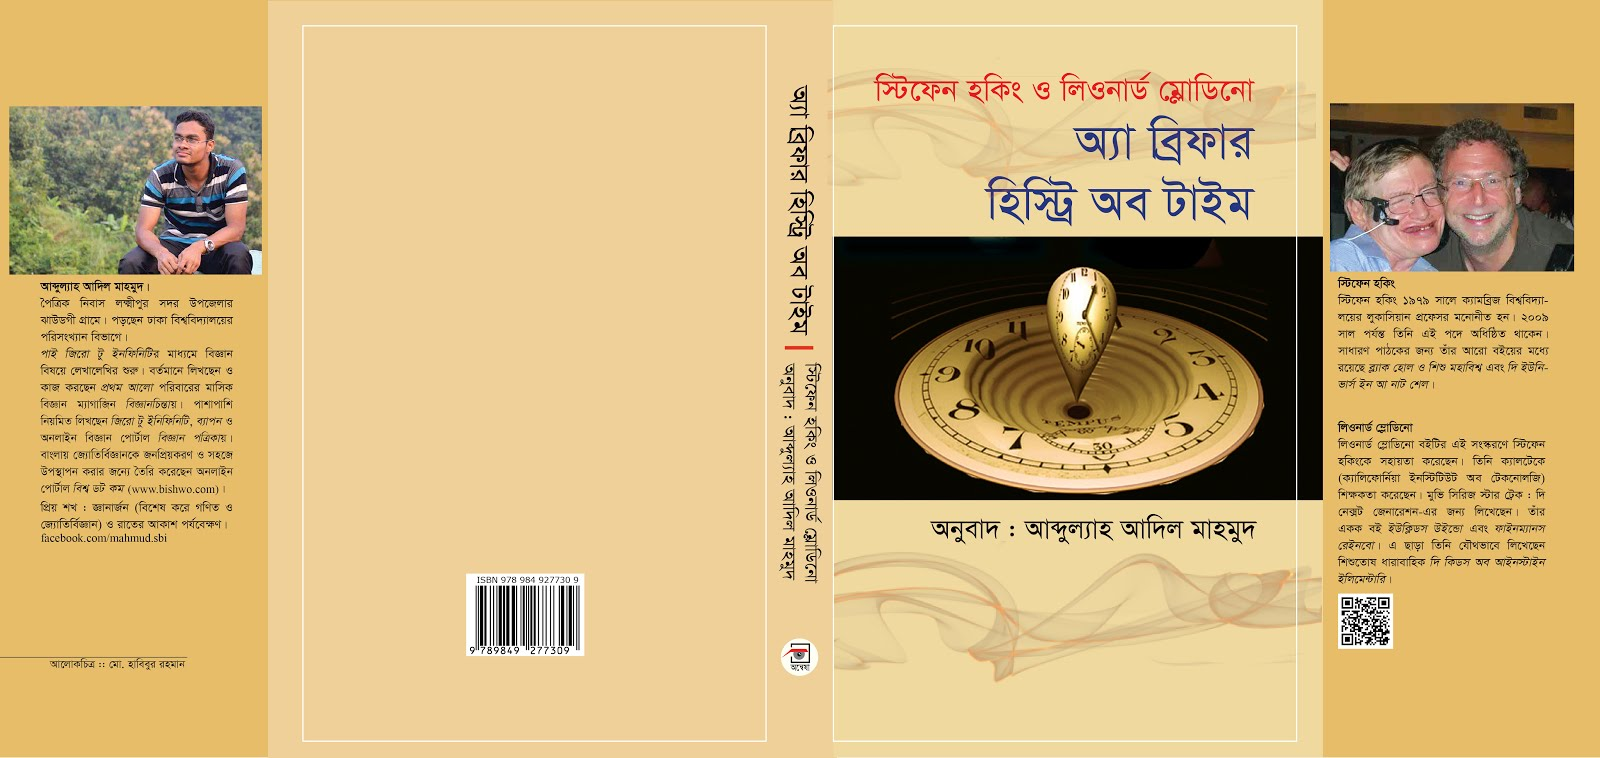
\includegraphics[width=0.6\linewidth]{img/books/briefer_history_of_time} 

}

\caption{A Briefer History of Time}\label{fig:abhot}
\end{figure}

\begin{figure}

{\centering 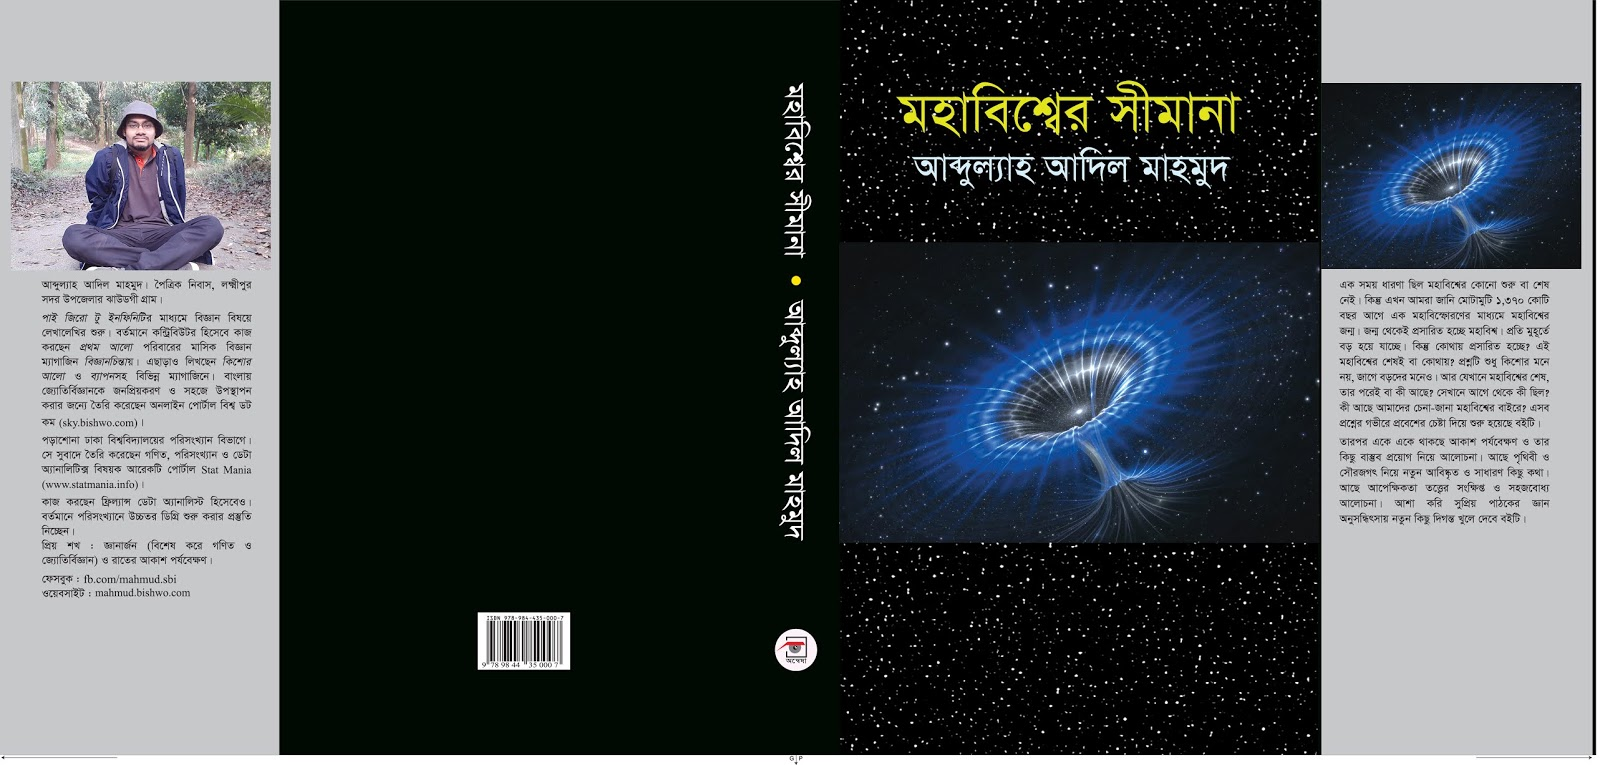
\includegraphics[width=0.6\linewidth]{img/books/ms} 

}

\caption{Mohabishwer Simana}\label{fig:ms}
\end{figure}

\begin{figure}

{\centering 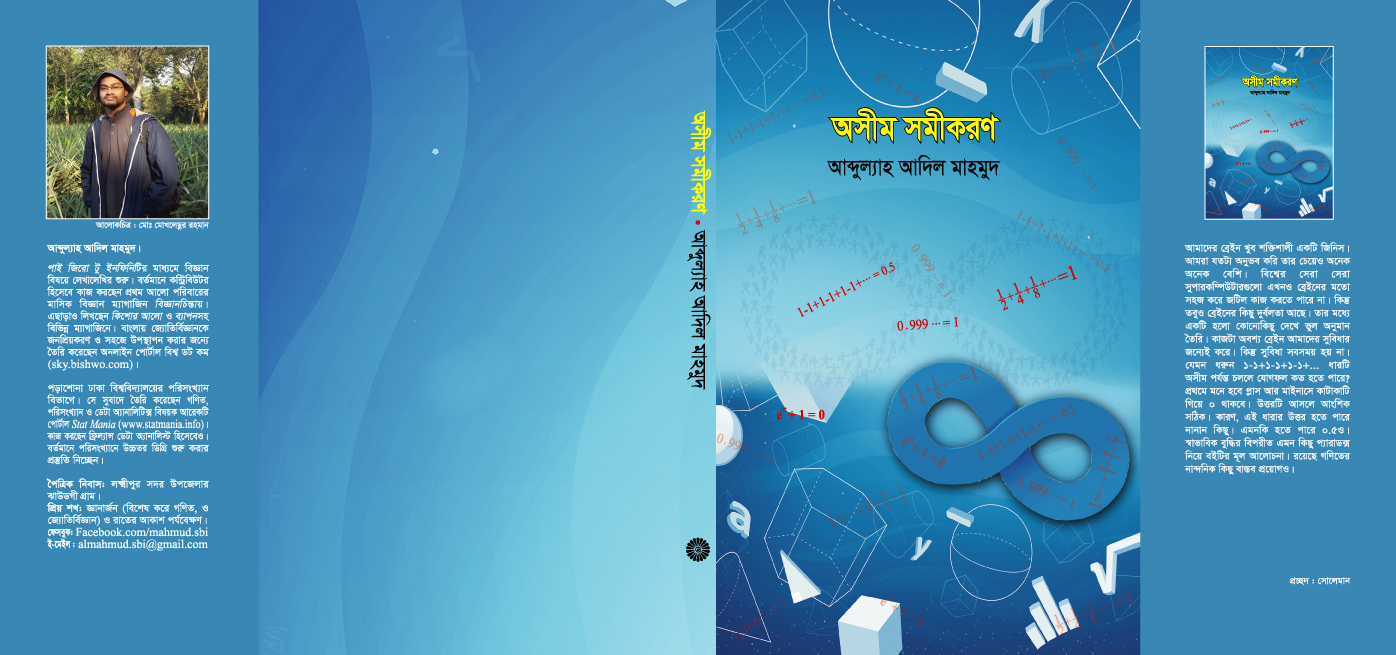
\includegraphics[width=0.6\linewidth]{img/books/cover_os} 

}

\caption{Osim Somikorn}\label{fig:os}
\end{figure}

\begin{figure}

{\centering 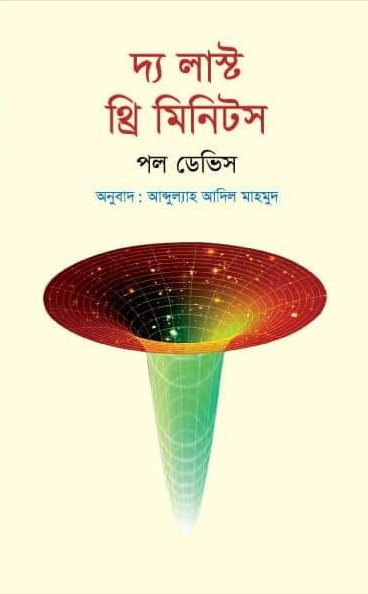
\includegraphics[width=0.6\linewidth]{books/images/books/l3m} 

}

\caption{The Last Three Minutes}\label{fig:l3m}
\end{figure}

\href{https://www.rokomari.com/book/author/47631}{Buy from Rokomari.com}

\hypertarget{gallery}{%
\chapter*{Gallery}\label{gallery}}
\addcontentsline{toc}{chapter}{Gallery}

\begin{figure}

{\centering 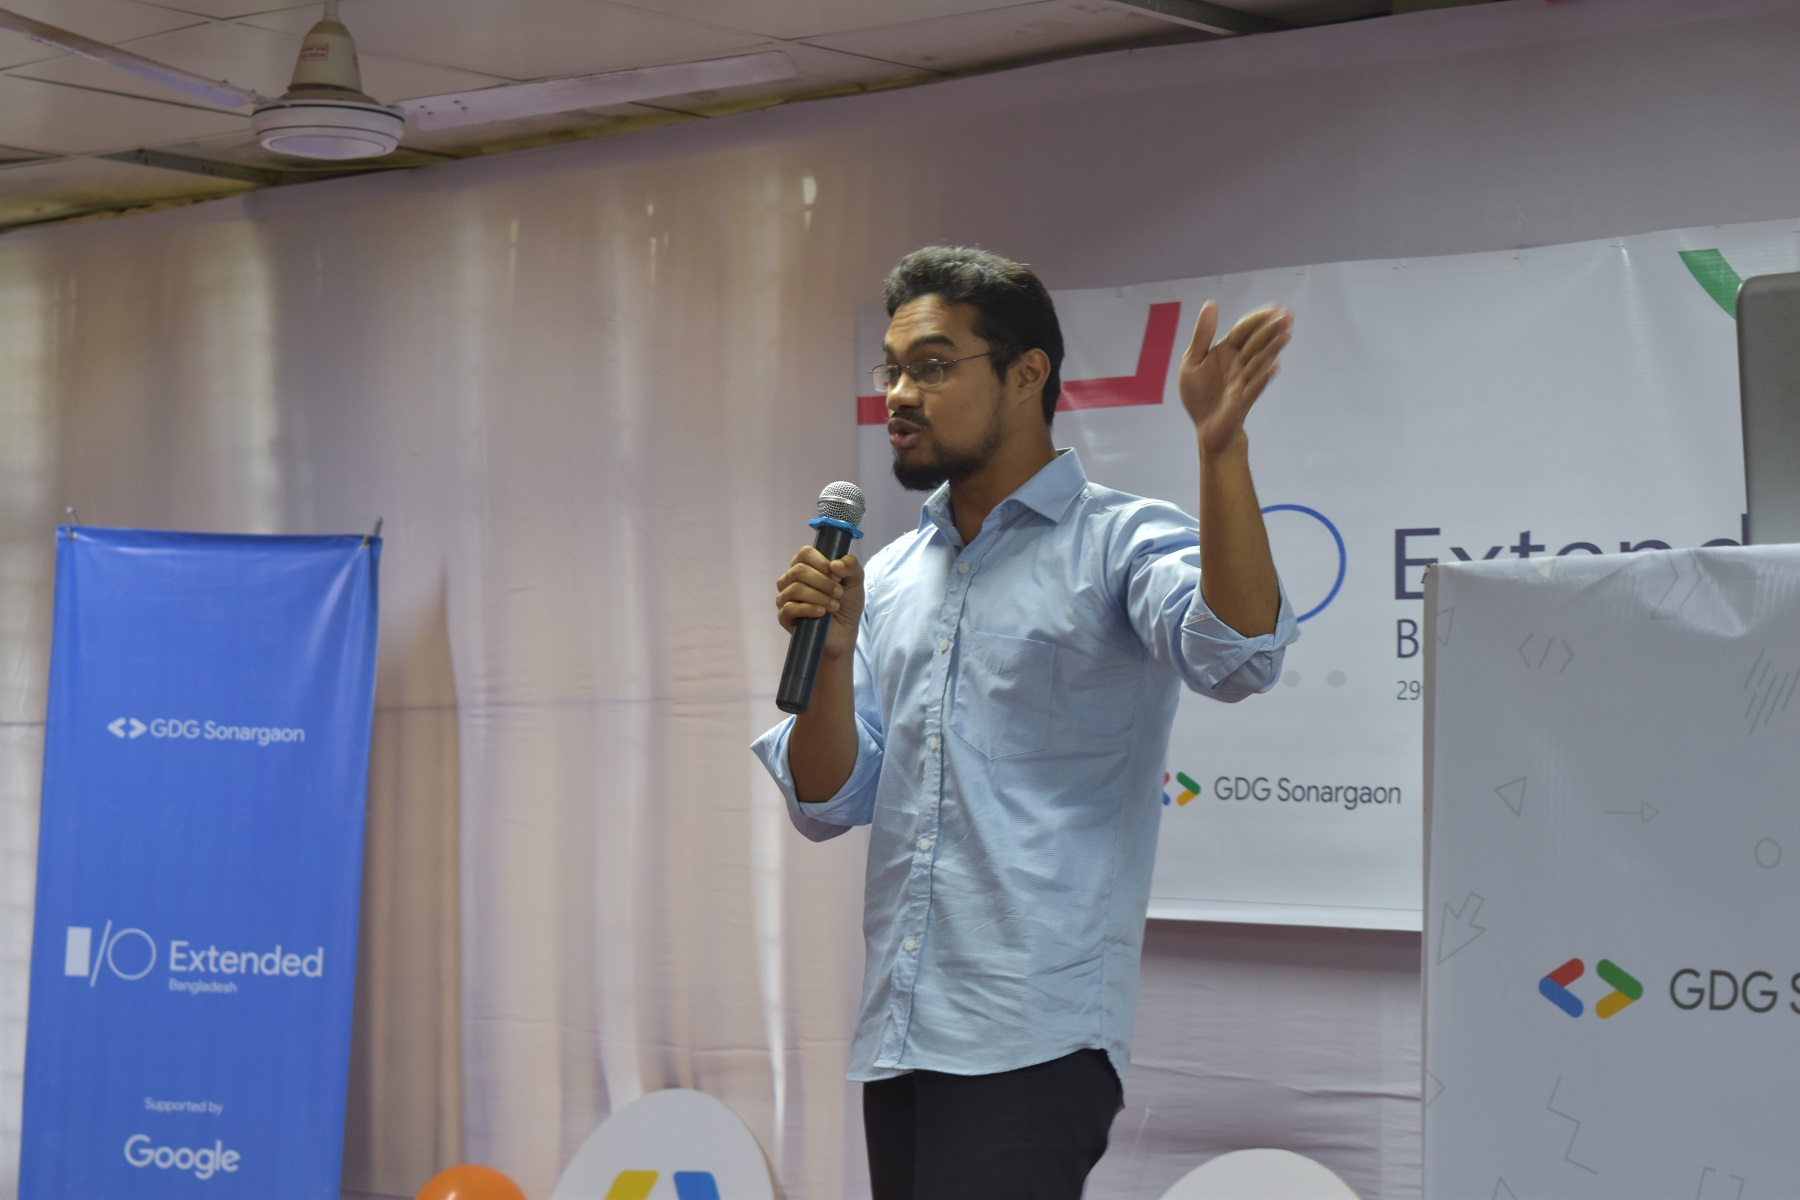
\includegraphics[width=0.6\linewidth]{img/miu1} 

}

\caption{Lecture At MIU.}\label{fig:miu}
\end{figure}

\begin{figure}

{\centering 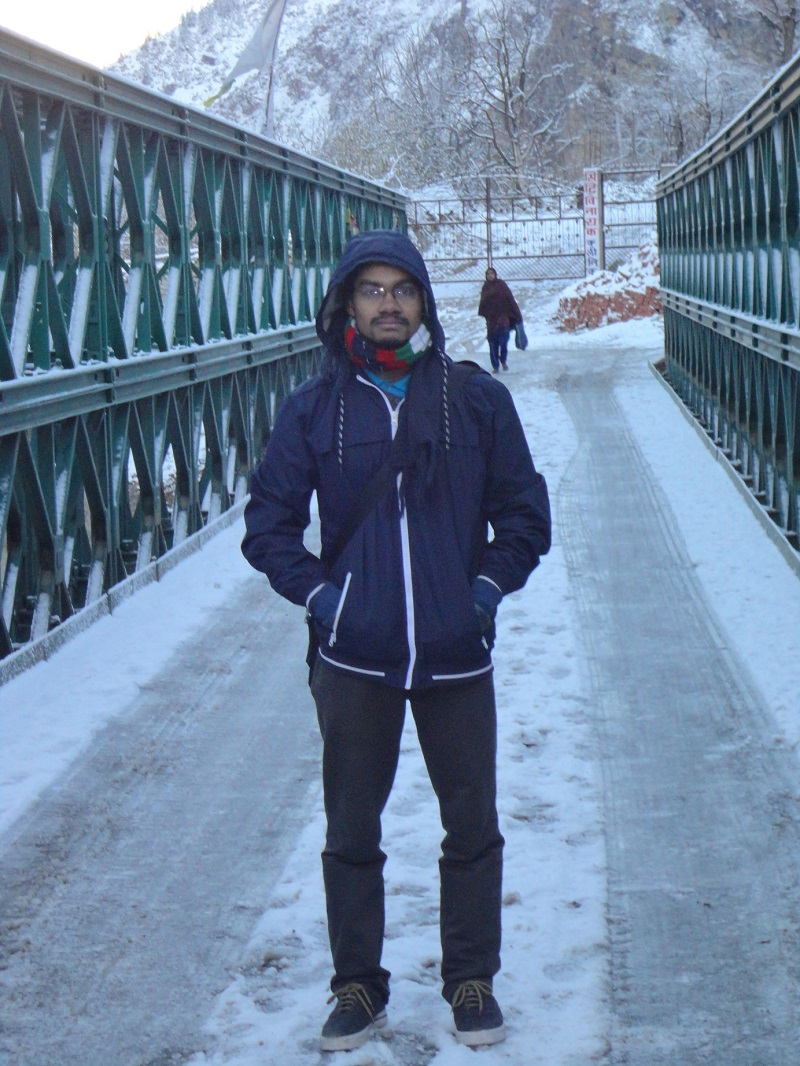
\includegraphics[width=0.6\linewidth]{img/sangla} 

}

\caption{Sangla, Kinnaur, Hiamchal Pradesh, India}\label{fig:sangla}
\end{figure}

\begin{figure}

{\centering 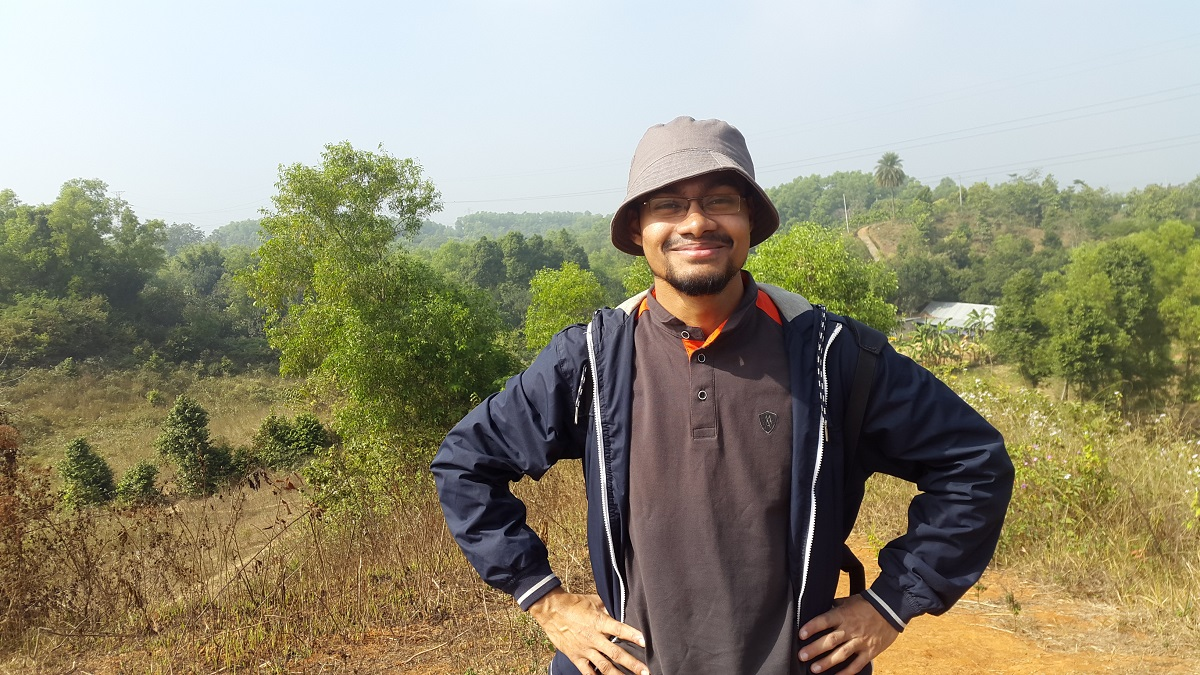
\includegraphics[width=0.6\linewidth]{img/lalmai} 

}

\caption{Roaming at Lalmai.}\label{fig:lal}
\end{figure}

\begin{figure}

{\centering 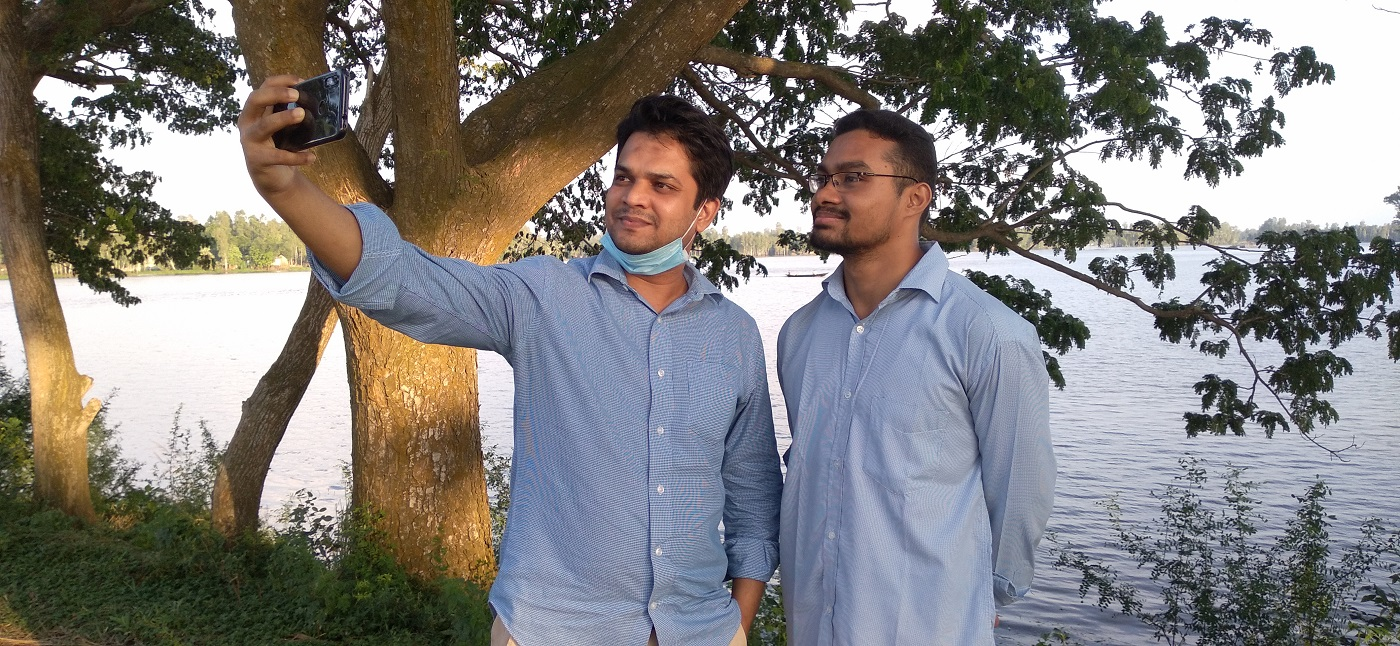
\includegraphics[width=0.6\linewidth]{img/cholonbil} 

}

\caption{Roaming at Cholonbil.}\label{fig:cbil}
\end{figure}

\begin{figure}

{\centering 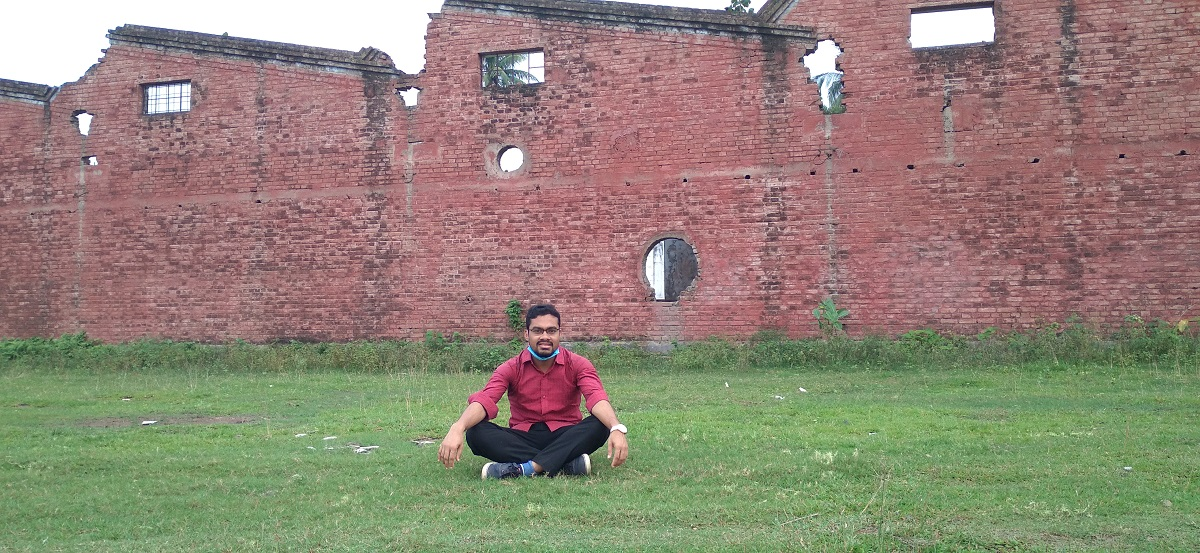
\includegraphics[width=0.6\linewidth]{img/pabna_mill} 

}

\caption{Roaming in Pabna.}\label{fig:mill}
\end{figure}

\hypertarget{websites}{%
\chapter*{Websites}\label{websites}}
\addcontentsline{toc}{chapter}{Websites}

\begin{itemize}
\tightlist
\item
  \href{https://lecture.statmania.info/}{Statistics Lectures}: Academic Lectures
\item
  \href{https://www.statmania.info/}{Stat Mania}: Web portal on statistics (esp.~with R programming) and mathematics, and Linux
\item
  \href{https://sky.bishwo.com}{মহাবিশ্ব}:Web portal on astronomy and cosmology
\item
  \href{https://lecture.statmania.info/pres.html}{Academic Lectures}
\item
  \href{https://rstat.statmania.info/}{R Programming Online}
\item
  \href{/blog}{Blog}
\end{itemize}

\hypertarget{contact}{%
\chapter*{Contact}\label{contact}}
\addcontentsline{toc}{chapter}{Contact}

\textbf{Email:} almahmud.sbi{[}at{]}gmail.com

\textbf{Facebook:} \href{https://www.facebook.com/mahmud.sbi}{mahmud.sbi}

\textbf{Linked In:} \href{https://www.linkedin.com/in/mahmudstat/t}{mahmudstat}

\hypertarget{resume}{%
\chapter*{Résumé}\label{resume}}
\addcontentsline{toc}{chapter}{Résumé}

See pdf (\href{cv/mahmud_cv_ac_latex.pdf}{academic}, \href{cv/mahmud_cv_pro_latex.pdf}{professional})

Abdullah Al Mahmud

\textbf{Lecturer in Statistics, Pabna Cadet College}

\begin{center}\rule{0.5\linewidth}{0.5pt}\end{center}

Contact Information

\textbf{Email:} almahmud.sbi{[}at{]}gmail.com

\textbf{Phone:} +880-1722-437040

\textbf{Github:} \href{https://github.com/mahmudstat}{\emph{mahmudstat}}

\textbf{Website:} \href{mahmud.statmania.info}{Stat Mania}

Employment History

\textbf{Lecturer in Statistics}

\begin{itemize}
\tightlist
\item
  \emph{Pabna Cadet College}
\item
  October, 2019 - Present
\end{itemize}

\textbf{Research Assistant}

\begin{itemize}
\tightlist
\item
  \emph{Engineers and Advisers Ltd.~(EAL)}
\item
  September, 2019 - October, 2019
\end{itemize}

Education

\textbf{MS in Statistics}

\begin{itemize}
\tightlist
\item
  University of Dhaka (2018-2019)
\item
  \textbf{CGPA}: 2.71 (out of 4)
\end{itemize}

\textbf{B.S. in Statistics}

\begin{itemize}
\tightlist
\item
  University of Dhaka (2012-2017)
\item
  \textbf{Project:} An Insight into Induced Seismicity in Bangladesh.
\item
  \textbf{Advisor:} Md. Ahsan Uddin
\item
  \textbf{CGPA:} 3.31 (out of 4)
\end{itemize}

\textbf{Higher Secondary School Certificate}

\begin{itemize}
\tightlist
\item
  Dhaka Board (July 2010)
\item
  Udayan Higher Secondary School
\item
  \textbf{GPA:} 5.00 (out of 5)
\end{itemize}

\textbf{Secondary School Certificate}

\begin{itemize}
\tightlist
\item
  Cumilla Board (May 2008)
\item
  Poura Shahid Smrity Academy
\item
  GPA: 5.00 (out of 5)
\end{itemize}

Test Scores

\begin{itemize}
\tightlist
\item
  \textbf{GRE:} 309 (\emph{Quantitative}: 160, \emph{Verbal}: 149)
\item
  \textbf{TOEFL:} 89 (\emph{Reading}: 24, \emph{Listening}: 21, \emph{Speaking}: 21 , \emph{Writing}: 23 )
\end{itemize}

Publications

\begin{enumerate}
\def\labelenumi{\arabic{enumi}.}
\tightlist
\item
  Mahmud, A, A . 2018. Testing of Compliance of Benford's Law with Disaster
  Death Tolls. Cadet College Journal.
\end{enumerate}

Conference Presentations

\begin{enumerate}
\def\labelenumi{\arabic{enumi}.}
\tightlist
\item
  Mahmud, A, A and Rahman, M, M. Goodness of fit for uniform distribution:
  Benford's law method. National Conference on Applications of Statistics on
  Sustainable Development Goals, MBSTU-2018, 24 September 2018. ID: TS3-11,
  Tangail, Bangladesh.
\end{enumerate}

Professional Researchers

\begin{enumerate}
\def\labelenumi{\arabic{enumi}.}
\tightlist
\item
  \textbf{Feasibility Study of Dhaka-Chattogram High-speed Rail Project}
\end{enumerate}

\begin{itemize}
\tightlist
\item
  November, 2018
\end{itemize}

\begin{enumerate}
\def\labelenumi{\arabic{enumi}.}
\setcounter{enumi}{1}
\tightlist
\item
  \textbf{Social Media Trend Analysis of Youth Students}
\end{enumerate}

\begin{itemize}
\tightlist
\item
  January, 2019
\end{itemize}

\begin{enumerate}
\def\labelenumi{\arabic{enumi}.}
\setcounter{enumi}{2}
\tightlist
\item
  Investment Prospect in Bangladesh (with EAL)
\end{enumerate}

\begin{itemize}
\tightlist
\item
  September, 2019
\end{itemize}

Other Reseacrhes

\begin{itemize}
\tightlist
\item
  \emph{An Insight into the Concept and Applictaions of Negative Probability}
\item
  \emph{Prediction of Rainfall Pattern in Bangladesh Using Machine Learning Algorithms}
\item
  \emph{An Insight into Induced Seismicity in Bangladesh}
\item
  \emph{Insight into And Application of Natural Randomness}
\end{itemize}

Science Books

\begin{enumerate}
\def\labelenumi{\arabic{enumi}.}
\tightlist
\item
  \href{https://www.rokomari.com/book/128479/a-briefer-history-of-time}{\textbf{Bengali Translation of \emph{A Briefer History of Time} }}
\end{enumerate}

\begin{itemize}
\tightlist
\item
  2017 Ekushey Book Fair
\item
  Authored by Stephen Hawking and Leonard Mlodino
\end{itemize}

\begin{enumerate}
\def\labelenumi{\arabic{enumi}.}
\setcounter{enumi}{1}
\tightlist
\item
  \href{https://www.rokomari.com/book/177345/mohabiswer-simana}{\textbf{Mohabishwer Simana (Edge of the Universe)}}
\end{enumerate}

\begin{itemize}
\tightlist
\item
  2019 Ekushey Book Fair
\end{itemize}

\begin{enumerate}
\def\labelenumi{\arabic{enumi}.}
\setcounter{enumi}{2}
\tightlist
\item
  \href{https://www.rokomari.com/book/179175/osim-somikoron}{\textbf{Osim Somikoron (The Infinite Equation)}}
\end{enumerate}

\begin{itemize}
\tightlist
\item
  2019 Ekushey Book Fair
\end{itemize}

\begin{enumerate}
\def\labelenumi{\arabic{enumi}.}
\setcounter{enumi}{3}
\tightlist
\item
  \href{https://www.rokomari.com/book/194398/chandrojoyer-50-bochor}{\textbf{Chondrojoyer 50 Bochor}}
\end{enumerate}

\begin{itemize}
\tightlist
\item
  2020 Ekushey Book Fair
\item
  Co-authored
\end{itemize}

\begin{enumerate}
\def\labelenumi{\arabic{enumi}.}
\setcounter{enumi}{4}
\tightlist
\item
  \href{https://l3m.bishwo.com/}{Translation of The Last Three Minutes*}
\end{enumerate}

\begin{itemize}
\tightlist
\item
  To be published in 2021 Ekushey Book Fair
\end{itemize}

Websites Developed

\begin{itemize}
\tightlist
\item
  \href{https://www.statmania.info}{\emph{Stat Mania}}
\item
  \href{https://rstat.statmania.info}{\emph{Statistics with R}}
\item
  \href{https://www.bishwo.com}{\emph{Bishwo.com}}
\item
  \href{https://os.statmania.info}{\emph{Osim Somikoron}}
\item
  \href{https://l3m.bishwo.com/}{\emph{The Last Three Minutes}}
\item
  \href{https://sky.bishwo.com}{\emph{Astronomy in Bengali}}
\end{itemize}

Technical Skills

Skills

\begin{itemize}
\tightlist
\item
  \emph{Programming Languages:} \texttt{R}, \texttt{Bash}, \texttt{FORTRAN}
\item
  \emph{Statistical Packages:} \texttt{STATA}, \texttt{SPSS}, \texttt{TABLEAU}
\item
  \emph{Database Management:} \texttt{SQL}
\item
  \emph{Geospatial Framework:} \texttt{GIS} (with \texttt{R})
\item
  \emph{Document Processing:} MS Office, Libreoffice, \texttt{Markdown}, \texttt{Latex}
\item
  \emph{Internet Skills:} \texttt{MathJax}, \texttt{HTML}, \texttt{CSS}, \texttt{SVG}, \texttt{JS}
\end{itemize}

Courses

\begin{enumerate}
\def\labelenumi{\arabic{enumi}.}
\tightlist
\item
  \href{https://www.coursera.org/learn/introduction-git-github/home/welcome}{\textbf{Introduction to Git and GitHub}}
\end{enumerate}

\begin{itemize}
\tightlist
\item
  Coursera
\item
  August 2020
\end{itemize}

\begin{enumerate}
\def\labelenumi{\arabic{enumi}.}
\setcounter{enumi}{1}
\tightlist
\item
  \href{https://www.coursera.org/learn/linux-tools-for-developers/home/welcome}{\textbf{Linux Tools for Developers}}
\end{enumerate}

\begin{itemize}
\tightlist
\item
  Coursera
\item
  May 2020
\end{itemize}

\begin{enumerate}
\def\labelenumi{\arabic{enumi}.}
\setcounter{enumi}{2}
\tightlist
\item
  \href{https://www.datacamp.com/courses/supervised-learning-in-r-classification}{\textbf{Supervised Learning in R: Classification}}
\end{enumerate}

\begin{itemize}
\tightlist
\item
  Data Camp
\item
  June 2018
\end{itemize}

Kaggle Competitions

\begin{itemize}
\item
  \textbf{Titanic: Machine Learning from Disaster}

  \emph{Accuracy}: 76.55\%
\item
  \textbf{Digit Recognizer}

  \emph{Accuracy}: 53\%
\item
  \textbf{House Price Prediction}

  \emph{Accuracy}: 92\%
\end{itemize}

Talks

\begin{enumerate}
\def\labelenumi{\arabic{enumi}.}
\tightlist
\item
  \textbf{Mathematics is Beautiful, So Is Programming}
\end{enumerate}

\begin{itemize}
\tightlist
\item
  \emph{MIU, 2018}
\end{itemize}

\begin{enumerate}
\def\labelenumi{\arabic{enumi}.}
\setcounter{enumi}{1}
\tightlist
\item
  \textbf{How to catch a Cheat Using Statistics}
\end{enumerate}

\begin{itemize}
\tightlist
\item
  \emph{Notre Dame College, 2017}
\end{itemize}

Workshops

\begin{itemize}
\tightlist
\item
  \textbf{July 2018:} \emph{Day long workshop on Statistics for Research by Dr.~Rahmatull Imon, professor, Ball State University, USA}
\item
  \textbf{December 2014:} \emph{Abdul Jabbar Workshop on Astronomy and Cosmology}
\item
  \textbf{June 2016:} \emph{Astronomy Workshop conducted by BAA and Russian Cultural
  Centre, Dhaka}
\end{itemize}

Extra-curricular Activities

\begin{itemize}
\tightlist
\item
  \emph{Member at Dhaka University Science Society (DUSS), University of Dhaka}
\item
  \emph{Writer at National Science Magazines, including BigganChinta}
\item
  \emph{Regular Public lectures on Mathematics and Astronomy}
\item
  \emph{Writing for Wikipedia}
\end{itemize}

Leadership Skills

\begin{itemize}
\tightlist
\item
  \emph{Led a team of 11 members in a research project in fourth year.}
\item
  \emph{Was a coordinator of Scholar's Forum, a student welfare organization.}
\item
  \emph{Coordinated Science Writers' cell, a platform of Bengali Science Writers.}
\end{itemize}

Language SKills

\begin{itemize}
\item
  \textbf{Bengali}

  \begin{itemize}
  \tightlist
  \item
    Mother Tongue
  \end{itemize}
\item
  \textbf{English}

  \begin{itemize}
  \tightlist
  \item
    Fluent in all areas
  \end{itemize}
\item
  \textbf{Arabic}

  \begin{itemize}
  \tightlist
  \item
    Introductory
  \end{itemize}
\end{itemize}

Résumé of Abdullah Al Mahmud

\end{document}
